\documentclass[10pt,a4paper]{article}
\usepackage[margin=19mm]{geometry}
\usepackage{amsmath,amssymb,graphicx,hyperref,array}
\hypersetup{colorlinks=true,urlcolor=blue,linkcolor=blue}
\setlength{\parindent}{0pt}\setlength{\parskip}{6pt}
\newcommand{\rw}{\mathord{\boldsymbol r\mkern2mu\wedge}}
\begin{document}
\begin{center}{\Large More public measurements for rigid-body contact}\\[5pt]
{Fixed material inputs, new comparisons and prediction readiness}\\[4pt]
October 7, 2026\end{center}

The project now has additional rubber-ball, sliding, non-spherical planar impact,
spatial impact and limestone rocking observations. This checkpoint holds published
material metadata fixed and exposes mismatches. It does not establish a complete
model that reproduces real collisions. No material coefficients were fitted here.

\textbf{Actual comparisons.} Errors below are predicted minus measured. Trial 1 is
an exploratory pilot in each GAUGE family/material and is excluded from evaluation.
Multiple samples/events within a trial are correlated. RMSE values for different
observables have different units and must not be pooled.

\begin{center}\small
\begin{tabular}{p{54mm}p{37mm}p{39mm}}\hline
Comparison & Evaluation amount & RMSE / maximum error\\\hline
Rubber bounce; observed impact marker & 42 events in 21 trials & 0.380733 / 0.671462 m/s\\
Wood sliding; nominal slope & 19 trials, 167 samples & 6.962 / 15.424 mm\\
Plastic sliding; nominal slope & 19 trials, 153 samples & 10.824 / 31.245 mm\\
Metal sliding; nominal slope & 18 trials, 158 samples & 2.880 / 7.771 mm\\
Limestone; ideal rocking geometry & 134 unique first events & 0.039013 / 0.125871 ratio\\\hline
\end{tabular}\end{center}

Sliding forecasts condition position and velocity on four initial moving samples,
then predict subsequent positions using fixed friction and gravity. The support
window ends before 0.30 m displacement from the initial sample. There are 59
released trials and 56 evaluation trials. The material values are unchanged;
their source field does not separately identify static and dynamic friction.

The bounce check conditions on an observed impact-marker timestamp, infers
incoming velocity from the incoming flight only, and compares the predicted
outgoing speed with an outgoing-only flight reconstruction at that timestamp.
It does not predict the contact time or use independently measured high-rate
contact states. The source restitution underpredicts the reconstructed response:
mean signed error -0.350346 m/s.

\textbf{State imports, not additional endpoint predictions.} MIT supplies 1,718
signed planar before/after states and contact Jacobians. GAUGE supplies 160 spatial
tetrahedron, wedge and pyramid trials: 280 body records and 4,686 pose samples.
These are now imported with explicit flat indices and units. Missing matched
coefficients, spatial inertia and contact-state uncertainty prevent a claim of
complete fixed-input prediction for these imports.

\textbf{Prediction status.} This is a normal-branch check, sustained-sliding
forecast, ideal-rocking comparator and data extension. The full directional
impulse/friction law and production solver have not been validated on these new
data. The attempted measured-angle correction worsens every sliding trial.

\newpage
\begin{center}{\large Deviations from measured reality}\end{center}
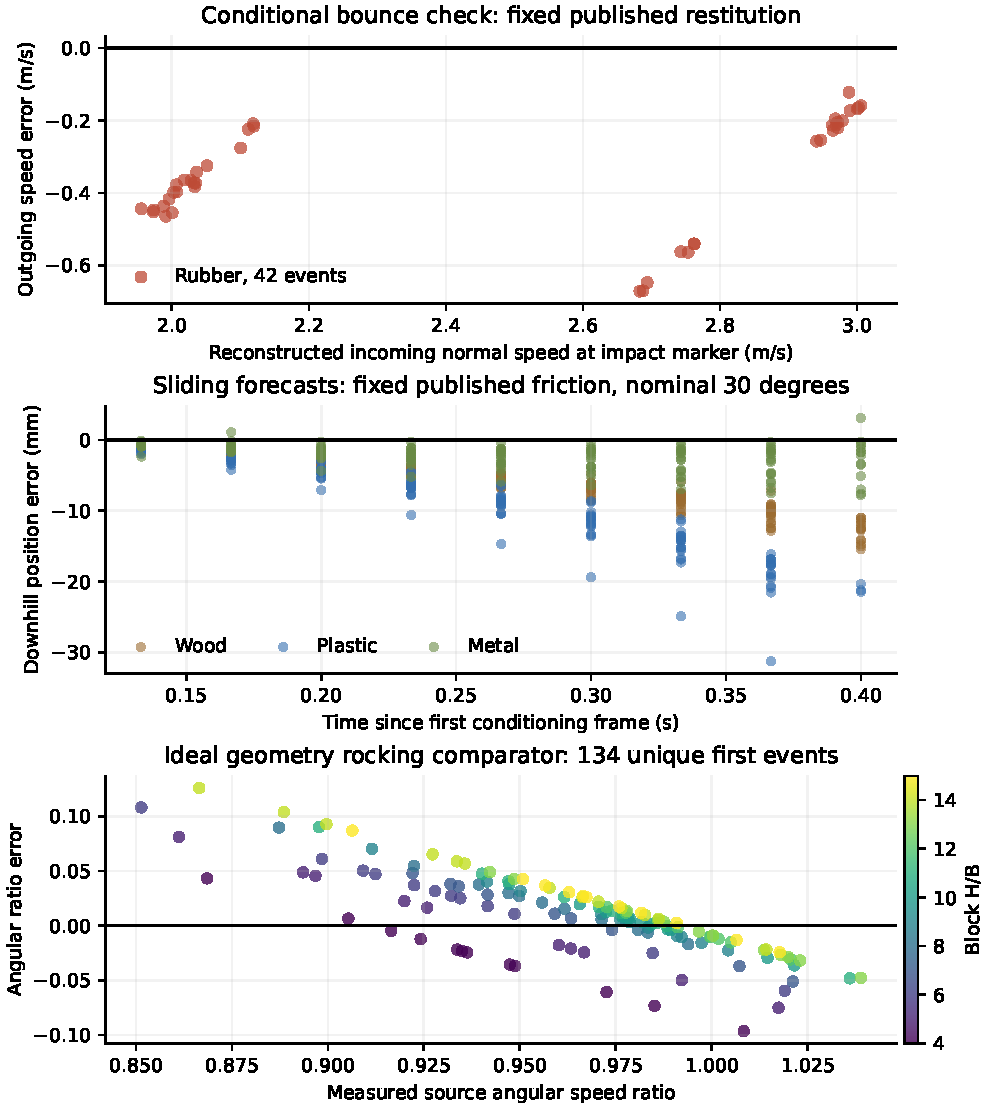
\includegraphics[width=\textwidth,height=201mm,keepaspectratio]{deviation-map.pdf}

The zero line means agreement. Colors distinguish materials or block geometry;
every admitted evaluation point is shown. Separate panels retain physical units.
Bounce and sliding are branch comparisons; the rocking panel is an established
ideal-geometry comparator. No bar charts or outcome-based removal of outliers.
The bounce timing envelope is discussed on the last page and is not drawn as a
statistical uncertainty band.

\newpage
\begin{center}{\large Published inputs and the failed correction}\end{center}
\begin{center}\small
\begin{tabular}{p{42mm}p{48mm}p{43mm}}\hline
Case & Values held fixed & Provenance / missing information\\\hline
GAUGE rubber & Mass 0.121 kg; source restitution 0.576733 & Generic restitution field; calibration-pair and split details incomplete\\
GAUGE sliders & Friction: wood 0.273673; plastic 0.275018; metal 0.262758 & Moving-branch interpretation; no separate $\mu_s$, $\mu_d$\\
MIT ellipse & Mass 0.0364 kg; semiaxes 0.035/0.025 m; gyration radius 0.0192 m & Reported planar $\mathbb I=1.3418496\,10^{-5}$ kg m$^2$; independent matched contact coefficients absent\\
Limestone blocks & Nominal dimensions, mass, geometric inertia & Effective geometry/ratios are outcomes; energy correction $f_c=0.7$ is assumed\\\hline
\end{tabular}\end{center}

In symbols, the two checked branches use
\[
 v_n^+=e_{\rm source}|v_n^-|,\qquad
 a=g\sin\theta-\mu g\cos\theta,\qquad
 x=x_0+v_0t+\tfrac12 at^2.
\]
Numerical material values are separate from the equations. Published scalar
fields do not automatically supply all normal/tangential restitution, static,
dynamic, rolling or spin resistance parameters of the full model.

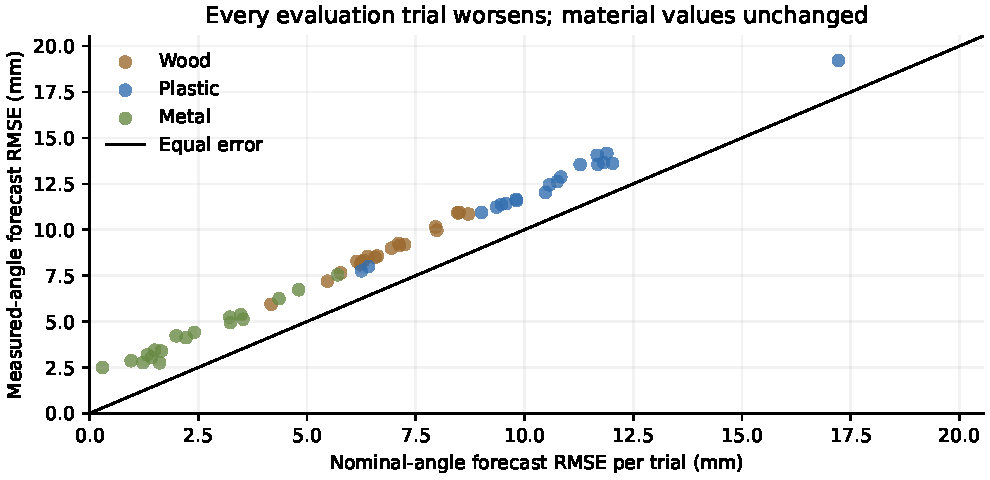
\includegraphics[width=\textwidth]{orientation-comparison.pdf}

The candidate uses board quaternions from the same four conditioning frames,
projects gravity onto the measured plane and leaves friction unchanged. Quaternion
and source Euler orientations agree within $1.74\,10^{-6}$ rad. Measured slopes
are 29.56--29.67 degrees. Candidate aggregate RMSE becomes 9.010/12.709/4.573 mm
(wood/plastic/metal), with \textbf{0/56 improved trials}. This correction cannot
explain the discrepancy. Retain the measured geometry and investigate contact or
calibration mismatch; do not change the angle or friction to hide the errors.

\newpage
\begin{center}{\large Non-spherical, spin and deformation challenges}\end{center}
\textbf{Planar ellipse impacts.} The signed pre/post translation and angular velocity
are directly useful for testing coupled momentum transfer. The source reports
250 Hz sampling and an experiment confined by a glass guide. Its supplied contact
Jacobians permit the diagnostic reconstruction
\[
 \Delta\boldsymbol p=m\Delta\boldsymbol v,\qquad
 \delta\boldsymbol L_{\rm residual}
 =\Delta\boldsymbol L-\rw\,\delta\boldsymbol p.
\]
The residual couple RMS is 0.00118023 N m s, but this is inferred from outcomes,
not independently measured contact torque. Finite-contact timing, contact-point
changes, gravity/external impulses, guide reactions and measurement noise can
contribute. Nominal ellipse geometry differs from the supplied contact Jacobians
by up to 1.72 mm. Do not identify the residual with a measured material coefficient.
The source authors fitted their model coefficients on these same data; those are
not independent inputs for our prediction test.

\textbf{Spatial tetrahedron, wedge and pyramid impacts.} All 160 released trials
are imported, not just schema pilots. Translation is converted from mm to m;
source quaternions remain in xyzw order, with norm error below $9\,10^{-7}$.
No measured full inertia tensor is supplied. Mesh-based homogeneous inertia would
be an explicit assumption. Source folder labels task-1/2/3 differ from metadata
task-3/4/5; restitution dictionaries are retained without an inferred mapping.
Full signed velocities and short contact intervals need uncertainty-aware
reconstruction before spatial endpoint testing.

\textbf{Limestone rocking.} Colombo et al.'s 2026 release contains 135 trial
folders, whereas its associated paper describes 120 tests. One processed pair,
BlockGroup\_1\_n13, exactly duplicates BlockGroup\_1\_n7. Keep both in the source
record but use only 134 unique first finite angular-ratio estimates for the primary
comparison. The ideal planar pivot-transfer comparator is
\[
 r_\omega=1-\frac{3B^2}{2(B^2+H^2)}.
\]
It requires ideal geometry and no sliding/bouncing. Ratios above one are retained:
22/134 primary outcomes and 2,820/7,519 finite unique-cycle estimates. These
processed ratios are not certified material restitution. Late-cycle estimates
are correlated and can be sensitive to small motions/processing. The archive also
contains raw 3D time histories; only processed summaries were used here.

\textbf{Compliant silicone and an ABS shell.} R\'emond et al. measure outgoing
spin for a 40 mm, 2.7 g shell on glass with silicone layers 0.50, 0.96, 1.25 and
1.78 mm thick. This is a useful challenge for small local shear/pressure history
instead of deforming every body. However, their friction near 0.92, effective mass
and local stiffness are fitted from rebound/spin results; derived moduli are not
independent characterization. Figure 8 has not yet been digitized here, so no new
prediction or numeric data count is claimed for this experiment.

The user model retains independent $\delta\boldsymbol L$, not just a lever moment,
and the full relative contact-velocity direction $\hat{\boldsymbol t}$ and spin
direction $\hat{\boldsymbol s}$. Conventional comparators do not resolve the
zero-slip directional closure or certify the complete implementation.

\newpage
\begin{center}{\large Measurement audit, reproducibility and next use}\end{center}
\textbf{Bounce input dependency corrected.} The original flight-intersection
reconstruction used both incoming and outgoing arcs to infer contact time.
Consequently the outgoing trajectory indirectly affected its reconstructed
incoming state. Its RMSE 0.382254 m/s is retained as a joint-arc consistency
diagnostic, not an independent endpoint prediction. The main table instead uses
the observed valley timestamp and incoming-only coefficients. This correction
was made after inspecting the initial outcomes; no pristine blind validation
is claimed. Restitution never changed.

Released GAUGE JSON is 30 Hz although the paper describes 180 Hz capture. A
conservative one-frame marker-time sensitivity for the signed speed error is
$\pm g(1+e_{\rm source})/30=\pm0.515592$ m/s. It spans zero for 35/42 corrected
errors. This envelope is not a confidence interval. Flight fits can be very good
without identifying true compression duration or deformable surface contact
height. Distinguish source-parameter mismatch from unresolved impact state and
boundary conditions before adopting a new friction/deformation law.

\textbf{Controls and preserved evidence.} Twenty-four analytic, instantaneous
bounce controls recover velocities within $1.47\,10^{-14}$ m/s; ballistic fits
within $1.34\,10^{-15}$. Nine plane/gravity controls pass. These validate the
extractor under its ideal assumptions. The MIT case/body-index naming correction
is independently checked across all 1,718 rows; physics, all other CSVs and metrics
are unchanged. Original evidence, protocols, hashes and source snapshots remain.

\textbf{Efficient representation.} The spatial import uses a flat case index,
one body index per case and explicit pose offsets/counts. Separate observed
position/quaternion channels can later feed Vektor Flow kernels without dense
pair-body tensors. This is data preparation, not a port, throughput benchmark or
group simulation. Earlier local contact-kernel benchmarks remain separate.

\textbf{Next experiment.} Resolve the GAUGE scene/material/subtask mapping;
reconstruct impact states with sampling and pose uncertainty; then compare the
current model with a passive, small local shear-history extension on declared
trial splits. Keep documented coefficients fixed. Missing-property estimation,
if needed, must have physical bounds and separate evaluation. Do not add an
arbitrary impulse polynomial or treat same-outcome fitted coefficients as public
independent material measurements. No empirical accuracy gain is claimed here.

\textbf{Primary sources.}\small
\begin{itemize}
\item Wang et al., \href{https://arxiv.org/html/2608.05948v1}{GAUGE (2026)};
\href{https://huggingface.co/datasets/InternRobotics/GAUGE-Dataset}{dataset}, MIT license.
\newline Pinned revision 9e0acb70fecc0d4161660264d9a4b08d8f56d45a.
\item Fazeli et al., \href{https://proceedings.mlr.press/v78/fazeli17a.html}{Learning Data-Efficient Rigid-Body Contact Models (2017)};
\href{https://github.com/mcubelab/planar-impact-dataset}{author dataset}.
\newline Pinned revision f24a7e3b31ad0b53652d6b2a6b26a702cc4362da.
Original MAT/code not redistributed here; derived observations attributed.
\item Colombo et al., \href{https://experiments.builtenvdata.eu/datasets/92/}{Free-rocking masonry dataset},
\href{https://doi.org/10.60756/uminho-jh25}{DOI 10.60756/uminho-jh25}, CC BY 4.0;
\href{https://link.springer.com/article/10.1007/s10518-025-02224-8}{associated paper}.
Archive SHA-256 a2423df131acf78692a18f8732d4054b1e87b5d798f8d322adb5d96d773952f4.
\item R\'emond et al., \href{https://data.hal.science/document/hal-05532284v1}{Effect of a compliant substrate on the rebound of a spherical shell (2026)},
\href{https://doi.org/10.1103/mmdr-2mm3}{DOI 10.1103/mmdr-2mm3}; original PDF outside package.
\end{itemize}
\normalsize Download receipts, per-row CSVs, flat pose arrays, scripts, protocols,
source catalog and this PDF accompany the report package. See the repository
README for reproduction commands. Original large archives remain in an external
cache. Scope: research-data extension; production physics unchanged.
\end{document}
